% Why agent-hub: a common agent loop next to the hub's flow. Compile with tectonic (XeTeX):
%   tectonic why_agent_hub.tex && pdftoppm -png -r 160 -singlefile why_agent_hub.pdf why_agent_hub
\documentclass[border=14pt]{standalone}
\usepackage{fontspec}
\setmainfont{Noto Sans}
\setsansfont{Noto Sans}
\setmonofont{DejaVu Sans Mono}[Scale=0.86]
\usepackage{tikz}
\usetikzlibrary{positioning,shapes.geometric,arrows.meta,calc,fit}
\definecolor{Ink}{HTML}{19334B}
\definecolor{Accent}{HTML}{11858A}
\definecolor{Muted}{HTML}{657482}
\definecolor{Warn}{HTML}{B03A2E}
\renewcommand{\familydefault}{\sfdefault}
\newcommand{\no}{\textcolor{Warn}{\textbf{\texttimes}}\ }
\newcommand{\badge}[1]{\tikz[baseline=(b.base)]\node[circle, fill=Accent, text=white, font=\scriptsize\bfseries, inner sep=1.3pt, minimum size=4.2mm] (b) {#1};}
\newcommand{\pt}[1]{\par\noindent\hangindent=1.3em\hangafter=1\makebox[1.3em][l]{\no}#1}

\begin{document}
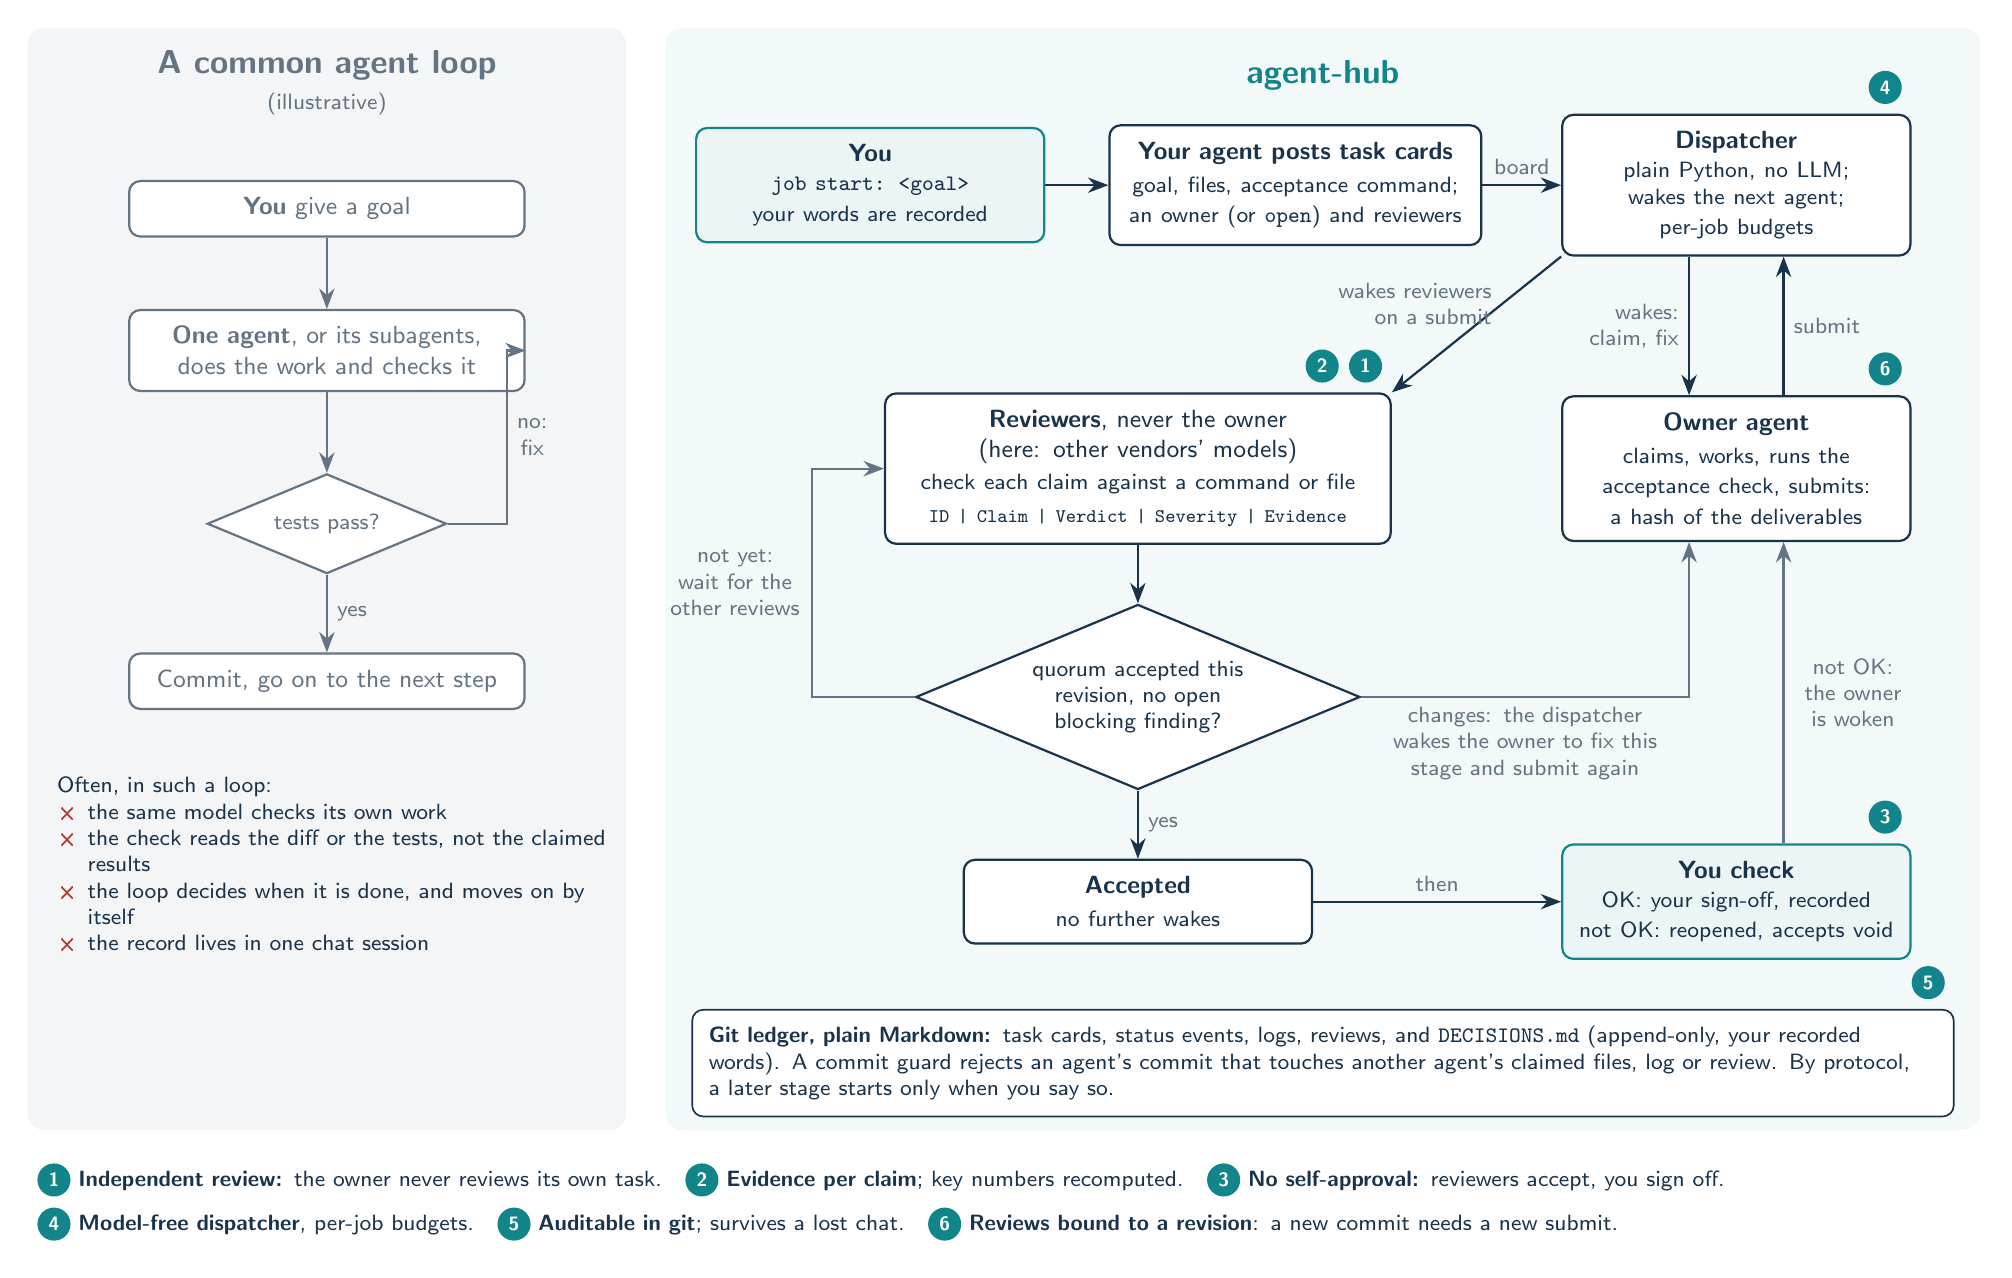
\begin{tikzpicture}[
  font=\small,
  box/.style={draw=Ink, line width=0.8pt, rounded corners=4pt, align=center, inner sep=6pt,
              fill=white, text=Ink},
  dull/.style={box, draw=Muted, text=Muted},
  you/.style={box, draw=Accent, fill=Accent!8},
  dec/.style={diamond, aspect=2.4, draw=Ink, line width=0.8pt, align=center, inner sep=1pt,
              fill=white, text=Ink, font=\footnotesize},
  arr/.style={-{Stealth[length=2.6mm]}, line width=0.8pt, draw=Ink},
  back/.style={-{Stealth[length=2.6mm]}, line width=0.8pt, draw=Muted},
  lab/.style={font=\footnotesize, text=Muted, align=center},
]
% ------------------------------------------------------------------ panels
\fill[Muted!7, rounded corners=6pt] (-0.2, 0.4) rectangle (7.4, -13.6);
\fill[Accent!5, rounded corners=6pt] (7.9, 0.4) rectangle (24.6, -13.6);
\node[font=\large\bfseries, text=Muted, align=center] at (3.6, -0.3) {A common agent loop\\[-1pt]{\footnotesize\mdseries (illustrative)}};
\node[font=\large\bfseries, text=Accent] at (16.25, -0.2) {agent-hub};

% ------------------------------------------------------------------ left: common loop
\node[dull, text width=4.6cm] (lyou) at (3.6, -1.9) {\textbf{You} give a goal};
\node[dull, text width=4.6cm] (lag) at (3.6, -3.7) {\textbf{One agent}, or its subagents,\\ does the work and checks it};
\node[dec, draw=Muted, text=Muted, text width=2.2cm] (ldec) at (3.6, -5.9) {tests pass?};
\node[dull, text width=4.6cm] (ldone) at (3.6, -7.9) {Commit, go on to the next step};
\draw[back] (lyou) -- (lag);
\draw[back] (lag) -- (ldec);
\draw[back] (ldec) -- node[lab, right] {yes} (ldone);
\draw[back] (ldec.east) -- ++(0.75,0) |- node[lab, right, pos=0.25] {no:\\fix} (lag.east);
\node[anchor=north west, text width=7.0cm, font=\footnotesize, text=Ink, align=left] at (0.05, -9.0) {
  Often, in such a loop:
  \pt{the same model checks its own work}
  \pt{the check reads the diff or the tests, not the claimed results}
  \pt{the loop decides when it is done, and moves on by itself}
  \pt{the record lives in one chat session}};

% ------------------------------------------------------------------ right: hub flow
\node[you, text width=4.0cm] (you) at (10.5, -1.6) {\textbf{You}\\[1pt]\footnotesize \texttt{job start: <goal>}\\ your words are recorded};
\node[box, text width=4.3cm] (post) at (15.9, -1.6) {\textbf{Your agent posts task cards}\\[1pt]\footnotesize goal, files, acceptance command; an owner (or \texttt{open}) and reviewers};
\node[box, text width=4.0cm] (disp) at (21.5, -1.6) {\textbf{Dispatcher}\\[1pt]\footnotesize plain Python, no LLM;\\ wakes the next agent;\\ per-job budgets};
\node[box, text width=4.0cm] (own) at (21.5, -5.2) {\textbf{Owner agent}\\[1pt]\footnotesize claims, works, runs the acceptance check, submits: a hash of the deliverables};
\node[box, text width=6.0cm] (rev) at (13.9, -5.2) {\textbf{Reviewers}, never the owner\\ (here: other vendors' models)\\[2pt]\footnotesize check each claim against a command or file\\[1pt] {\scriptsize\texttt{ID | Claim | Verdict | Severity | Evidence}}};
\node[dec, text width=3.2cm] (dec) at (13.9, -8.1) {quorum accepted this\\ revision, no open\\ blocking finding?};
\node[box, text width=4.0cm] (acc) at (13.9, -10.7) {\textbf{Accepted}\\[1pt]\footnotesize no further wakes};
\node[you, text width=4.0cm] (chk) at (21.5, -10.7) {\textbf{You check}\\[1pt]\footnotesize OK: your sign-off, recorded\\ not OK: reopened, accepts void};

\draw[arr] (you) -- (post);
\draw[arr] (post) -- node[lab, above] {board} (disp);
\draw[arr] ($(disp.south)+(-0.6,0)$) -- node[lab, left, align=right] {wakes:\\claim, fix} ($(own.north)+(-0.6,0)$);
\draw[arr] ($(own.north)+(0.6,0)$) -- node[lab, right] {submit} ($(disp.south)+(0.6,0)$);
\draw[arr] (disp.south west) -- node[lab, left, pos=0.35, align=right] {wakes reviewers\\ on a submit} (rev.north east);
\draw[arr] (rev) -- (dec);
\draw[arr] (dec) -- node[lab, right] {yes} (acc);
\draw[arr] (acc) -- node[lab, above] {then} (chk);
\draw[back] (dec.west) -- ++(-1.3,0) |- node[lab, left, pos=0.25, text width=1.7cm] {not yet:\\ wait for the other reviews} (rev.west);
\draw[back] (dec.east) -| node[lab, below, pos=0.25, text width=4.0cm] {changes: the dispatcher wakes the owner to fix this stage and submit again} ($(own.south)+(-0.6,0)$);
\draw[back] ($(chk.north)+(0.6,0)$) -- node[lab, right, text width=1.5cm] {not OK: the owner is woken} ($(own.south)+(0.6,0)$);

% ledger
\node[draw=Ink, line width=0.6pt, rounded corners=4pt, fill=white, text=Ink, align=left,
      text width=15.6cm, inner sep=6pt, font=\footnotesize] (led) at (16.25, -12.75) {
  \textbf{Git ledger, plain Markdown:} task cards, status events, logs, reviews, and \texttt{DECISIONS.md}
  (append-only, your recorded words). A commit guard rejects an agent's commit that touches another
  agent's claimed files, log or review. By protocol, a later stage starts only when you say so.};

% badges on the right flow
\node[anchor=south east] at (rev.north east) {\badge{1}};
\node[anchor=south east] at ($(rev.north east)+(-0.55,0)$) {\badge{2}};
\node[anchor=south east] at (disp.north east) {\badge{4}};
\node[anchor=south east] at (chk.north east) {\badge{3}};
\node[anchor=south east] at (led.north east) {\badge{5}};
\node[anchor=south east] at (own.north east) {\badge{6}};

% ------------------------------------------------------------------ legend of advantages
\node[anchor=north west, text width=24.6cm, align=left, font=\footnotesize, text=Ink] at (-0.2, -13.9) {
  \badge{1} \textbf{Independent review:} the owner never reviews its own task.\quad
  \badge{2} \textbf{Evidence per claim}; key numbers recomputed.\quad
  \badge{3} \textbf{No self-approval:} reviewers accept, you sign off.\\[3pt]
  \badge{4} \textbf{Model-free dispatcher}, per-job budgets.\quad
  \badge{5} \textbf{Auditable in git}; survives a lost chat.\quad
  \badge{6} \textbf{Reviews bound to a revision}: a new commit needs a new submit.};
\end{tikzpicture}
\end{document}
